\documentclass[sigconf]{acmart}

\usepackage{booktabs} % For formal tables


% Copyright
%\setcopyright{none}
%\setcopyright{acmcopyright}
%\setcopyright{acmlicensed}
\setcopyright{rightsretained}
%\setcopyright{usgov}
%\setcopyright{usgovmixed}
%\setcopyright{cagov}
%\setcopyright{cagovmixed}


% DOI
%\acmDOI{10.475/123_4}
%
%% ISBN
%\acmISBN{123-4567-24-567/08/06}

%Conference
\acmConference[PEARC'18]{Practice and Experience in Advanced Research Computing}{July 2018}{Pittsburgh, PA, USA}
\acmYear{2018}
\copyrightyear{2018}
%
%
%\acmArticle{4}
%\acmPrice{15.00}

% These commands are optional
%\acmBooktitle{Transactions of the ACM Woodstock conference}
%\editor{Jennifer B. Sartor}
%\editor{Theo D'Hondt}
%\editor{Wolfgang De Meuter}


\begin{document}
\title{The CSBG - LSU Gateway: Web based Hosted Gateway for Computational System Biology Application Tools from Louisiana State University}

\author{Eroma Abeysinghe}
\affiliation{%
  \institution{Pervasive Technology Institute, Indiana University}
}
\email{eabeysin@iu.edu}

\author{Michal Brylinski}
\affiliation{%
  \institution{Department of Biological Sciences, Louisiana State University}
}
\email{michal@brylinski.org}

\author{Marcus Christie}
\affiliation{%
  \institution{Pervasive Technology Institute, Indiana University}
}
\email{machrist@iu.edu}

\author{Suresh Marru}
\affiliation{%
  \institution{Pervasive Technology Institute, Indiana University}
}
\email{smarru@iu.edu}

\author{Marlon Pierce}
\affiliation{%
  \institution{Pervasive Technology Institute, Indiana University}
}
\email{marpierc@iu.edu}

\begin{abstract}
Science gateways are identified as an effective way to publish and distribute software for research communities without the burden of learning HPC (High Performance Computer) systems. In the past, researchers were expected to have in-depth knowledge on using HPC systems for computations along with  their respective science field in order to do effective research. Science gateways eliminates the need to learn HPC systems and allows the research communities to focus more on their science and let the gateway handle communicating with HPCs. In this poster we are presenting the science gateway project of CSBG (Computational System Biology Group - www.brylinski.org) of  Department of Biological Sciences with Center for Computation \& Technology at LSU (Louisiana State University). The gateway project was initiated in order to provide CSBG software tools as a service through a science gateway.
\end{abstract}

%
% The code below should be generated by the tool at
% http://dl.acm.org/ccs.cfm
% Please copy and paste the code instead of the example below.
%
\begin{CCSXML}
<ccs2012>
<concept>
<concept_id>10010147.10010341.10010370</concept_id>
<concept_desc>Computing methodologies~Simulation evaluation</concept_desc>
<concept_significance>500</concept_significance>
</concept>
<concept>
<concept_id>10011007.10011074.10011075.10011077</concept_id>
<concept_desc>Software and its engineering~Software design engineering</concept_desc>
<concept_significance>300</concept_significance>
</concept>
</ccs2012>
\end{CCSXML}

\ccsdesc[500]{Computing methodologies~Simulation evaluation}
\ccsdesc[300]{Software and its engineering~Software design engineering}

\keywords{Apache Airavata, Science Gateway, Computational System Biology}

\maketitle

\section{Introduction}

The Computational System Biology Group (CSBG) at LSU with consultation and development support from the Science Gateways Community Institute (SGCI) ~\cite{sgci} are developing the www.sciencegateway.brylinski.org gateway for existing and new users of CSBG tools. Currently the group has about half a dozen software tools developed and in production. They are compiled and installed in LSU cluster (mike.hpc.lsu.edu) with plans expanding to the SuperMIC XSEDE cluster (smic.hpc.lsu.edu). The gateway is envisioned to be practical in terms of reaching large number of users and managing them through the gateway as well as a way to reduce the number of errors and issues of individuals compiling and installing the software on their own. 

\section{CSBG  TOOLS}
CSBG offers a variety of tools for Structural Bioinformatics to support the prediction of protein structure and function from raw sequence data. eThread is a meta-threading procedure to accurately identify templates for protein modeling and functional annotation. This tool was shown to outperform single-threading approaches generating models correctly at the fold level for the majority of targets and detecting many facets of protein function even in a low sequence identity regime. Improved template selection by eThread motivated us to develop eFindSite, a method for ligand-binding site and residue prediction. eFindSite employs various machine learning techniques to efficiently integrate structural and evolutionary information. It has been shown to provide more accurate annotations than other methods for ligand-binding site and residue prediction. An example of the modeled structure of a gene product from the human proteome by eThread with a drug-binding site annotated by eFindSite is shown in Figure 1.

\begin{figure}
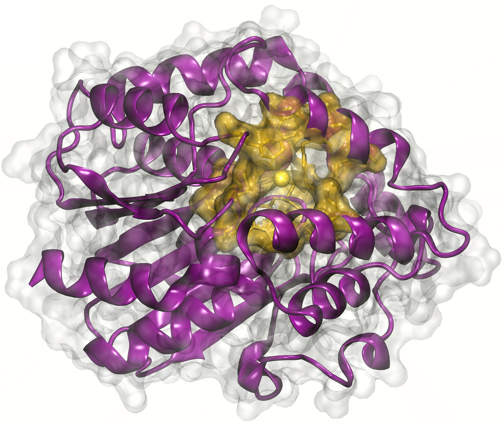
\includegraphics[height=3in, width=3.5in]{Fig1-protein-structure.png}
\caption{Example of a protein structure modeled with eThread (purple) and putative drug-binding site predicted with eFindSite (gold)}
\end{figure}

eSimDock is a similarity-based docking tool employing non-linear machine learning-based scoring functions to improve the accuracy of ligand ranking and binding pose prediction. Importantly, the performance of eSimDock is largely unaffected by the deformation of ligand binding regions; thus it represents a practical strategy for across-proteome virtual screening against protein models. Moreover, we developed another ligand docking algorithm, GeauxDock, which uses a descriptor-based scoring function integrating evolutionary constraints with physics-based energy terms. GeauxDock is well suited for proteome-scale applications taking advantage of the increasingly growing protein sequence and structural data.

eFindSitePPI and eRankPPI are programs to predict protein-binding interfaces and assembly dimer structures. eFindSitePPI uses the 3D structure of a target protein, remotely related templates and machine learning to predict binding residues. A unique feature of eFindSitePPI is its capability to detect specific molecular interactions at the interface. eRankPPI is an algorithm for the identification of near-native conformations generated by protein docking using experimental structures as well as protein models. It employs multiple features including interface probability estimates calculated by eFindSitePPI and a novel contact-based symmetry score. Both programs were demonstrated to consistently outperform other algorithms, offering a high accuracy in the exhaustive structure-based reconstruction of protein-protein interaction networks across proteomes. 


\section{CSBG USERS}

There is a growing interest in our tools from the research community. Existing web servers have been used by other groups to process 3,103 jobs since 2012. Figure 2 shows the number of jobs submitted each month. For instance, eThread and eFindSite have been used 754 and 1,476 times, respectively. The majority of users are experimental groups with limited experience in processing jobs on HPC machines. Science gateways provide an easy access to CSBG tools, which can be used to support a number of projects ranging from across-proteome function inference to drug discovery.

\begin{figure}
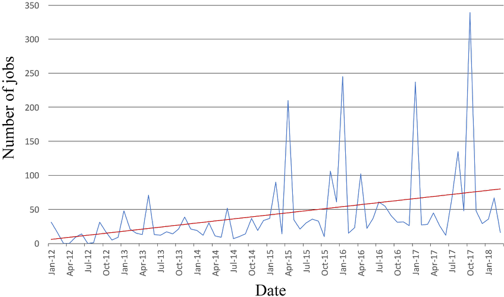
\includegraphics[height=3in, width=3.5in]{Fig2-usage.png}
\caption{Number of jobs submitted by external users each month (blue). Red is the trendline.}
\end{figure}

\section{CSBG GATEWAY WITH SCIGAP SERVICES}

\subsubsection{Design \& Implementation}
CSBG contacted SGCI for support for gateway project. Through SGCI, the project was assigned to the SciGaP ~\cite{scigap} gateway team. The multi-tenanted SciGaP gateway platform provides hosted, managed gateway portals for science communities with data storage for user data files. SciGaP provides primary services required by a science gateway, user identity management, accounts, authorization, and access to multiple high performance computer (HPC) resources from campus, national, and international resource providers. The SciGaP platform uses Apache Airavata ~\cite{airavata} middleware for computational job construction, submission to HPCs and to manage computational execution data files, inputs and outputs. The CSBG Gateway consists of a web client for end users to communicate with the LSU cluster and XSEDE cluster and dedicated data storage for gateway user data. The gateway client, gateway storage resource and Apache Airavata middleware are hosted at Indiana University. Figure  3 depicts the aforementioned set up of gateway web client, gateway middleware components with HPC clusters.

\subsubsection{Planning and Configuration}
CSBG required customizations on top of the default gateway web client provided by the SciGaP services. Customizations mainly focused on minimizing erroneous data uploading for bioinformatic softwares. Users uploading erroneous data can result in HPC resource and time wastage and also blocking the other users from using the HPCs due to traffic. To do so, it was discussed and designed to validate data inputs prior to experiment submission in the gateway. The ?Experiment? is the record created and launched in the gateway in order to create a job script and submit the job to the HPC cluster. Validations are done when user adds the inputs required for software execution. Instead of uploading a single large input file with all the data required to execute the software, the input is absorbed in the formats of input text, selecting from option buttons, checkboxes, etc. Options are nested; based on previously selected options, the current options can change. The CSBG gateway supports configuring the bioinformatic softwares with required validations. Gateway admin can add validations for each input field at the time of configuring the application.
Gateway is currently configured to run bioinformatic computations on LSU SuperMike-II cluster and can expand to any XSEDE cluster. 

\subsection{User Access}
The CSBG gateway has the option of letting users use already existing organizational accounts (e.g.: Google, campus login, etc...) to gain access or create a new gateway user account. Apache Airavata uses open source Keycloak ~\cite{christie2017using} identity management system for user account creation and to authorize and authenticate.  CILogon ~\cite{basney2014cilogon} is the federated authentication system used to enable using other organizational logins to create a gateway account. Gateway administrators can decide on the level of access to the gateway that they want to grant users. 

Another requirement for CSBG Gateway is to have ?guest?, or ?anonymous? gateway login. These accounts are to be used by potential users who want to explore the gateway or researchers or reviewers of journal and paper submissions. Such user accounts ensure access to the gateway without revealing personal data such as name, email, and institute. While such accounts are practical from guest or temporarily user point of view, the gateway administrator would want to provide restricted access on using SuperMike for test type computations.  As a result, the gateway development team is currently working on providing restricted access to the gateway in terms of  software and HPC usage. 

\subsection{ Secure Communication}
Apache Airavata uses SSH key based communication with HPCs and user data storage at the gateway client side. Gateway credential store ~\cite{kanewala2014credential} allows the gateway admin to generate public-private key pairs to be used for secure communications. Gateway administrators can create as many as needed, either use one key for all communications or have dedicated keys created for each cluster and data storage. These channels are used for computational job script transfer from Airavata middleware to the cluster working directory, input  and output data transfers from gateway data storage to the cluster.

\subsection{Bioinformatic Computations}

Two bioinformatic tools, eThread and eFindSite by CSBG are currently available within the gateway for users. In order to use them users need to provide the required inputs and launch an ?experiment? in the gateway. The ?experiment? will submit a job script with all required information to run together with data files uploaded by the user. 

\begin{figure}
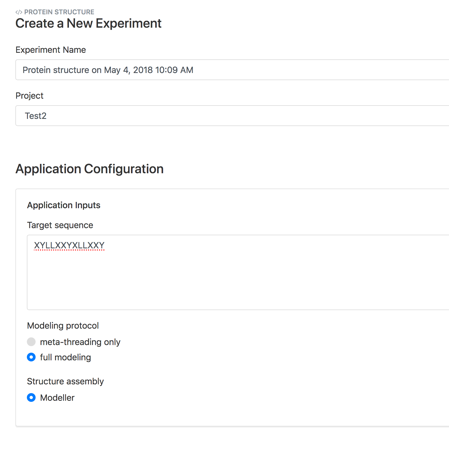
\includegraphics[height=3in, width=3.5in]{Fig3-experiment-launch.png}
\caption{eThread Experiment Launch Page.}
\end{figure}

\section{OUTREACH EVENTS}

We plan to disseminate gateways to a broad research community. The online resources will include comprehensive sets of manuals, tutorials and various case studies to encourage and help others adopt our tools in their projects. We will not only actively promote scientific gateways at various conferences, but also use these tools in the classroom. Protein structure modeling and functional inference will be included in several courses currently offered at LSU for undergraduate and graduate students. These efforts will increase the student awareness of the importance of computational approaches to modern biological research.

\section{Conclusions}
The CSBG group will keep enhancing and improving the current software tools they have and they will be made available from www.sciencegateway.brylinski.org. Currently it is planned to be available on SuperMIC but going forward it will be expanded, and users will have the option of selecting where to run the jobs from a wide range of HPCs ranging from campus to national, XSEDE resources. The gateway is planned to be introduced and used in classroom environments and also expanding the horizon with new users who needs to use bioinformatics softwares without the hassle of needing to learn ways of HPCs. 

%\end{document}  % This is where a 'short' article might terminate


\begin{acks}
The Louisiana State University - Computational System Biology Group Science Gateway was implemented with the support from the Science Gateways Community Institute (NSF award 1547611). Development of the Apache Airavata used to develop the science gateway is supported by NSF award 1339774. 

\end{acks}

\bibliographystyle{ACM-Reference-Format}
\bibliography{csgb-lsu-pearc18-abstract}

\end{document}
